% !TEX program = xelatex
% Biên dịch: xelatex bao_cao_de_tai_8.tex (chạy 2 lần để có mục lục)
% Các ô {\color{red}[...]} là chỗ cần điền số liệu sau khi chạy dropout_pipeline.py.

\documentclass[12pt,a4paper]{article}

\usepackage{fontspec}
\setmainfont{Times New Roman}
\usepackage[vietnamese]{babel}
\usepackage[a4paper,top=2.5cm,bottom=2.5cm,left=3cm,right=2cm]{geometry}
\usepackage{graphicx}
\usepackage{booktabs}
\usepackage{array}
\usepackage{amsmath}
\usepackage{float}
\usepackage{caption}
\usepackage{enumitem}
\usepackage{xcolor}
\usepackage{listings}
\usepackage[hidelinks]{hyperref}

\graphicspath{{results/}}
\setlength{\parskip}{0.4em}
\setlength{\parindent}{1.2em}
\linespread{1.2}

\lstset{
  language=Python,
  basicstyle=\ttfamily\small,
  breaklines=true,
  frame=single,
  numbers=left,
  numberstyle=\tiny,
  keywordstyle=\color{blue!70!black}\bfseries,
  commentstyle=\color{green!40!black},
  showstringspaces=false,
  captionpos=b,
}

\newcommand{\ph}[1]{{\color{red}[#1]}}

\begin{document}

% ------------------------------------------------------------------
% TRANG BÌA
% ------------------------------------------------------------------
\begin{titlepage}
\centering
{\large TRƯỜNG ĐẠI HỌC ĐẠI NAM}\\[0.3cm]
{\large KHOA CÔNG NGHỆ THÔNG TIN}\\[2cm]
{\Large\bfseries BÁO CÁO BÀI TẬP LỚN}\\[0.3cm]
{\large HỌC PHẦN NHẬP MÔN HỌC MÁY (FIT4013)}\\[1.5cm]
{\Large\bfseries ĐỀ TÀI 8: DỰ ĐOÁN SINH VIÊN CÓ NGUY CƠ BỎ HỌC}\\[0.5cm]
{\large Dữ liệu: UCI 697 — Predict Students' Dropout and Academic Success}\\[2.5cm]
\begin{tabular}{rl}
Giảng viên hướng dẫn: & ThS. Lê Thị Thùy Trang\\
Nhóm thực hiện: & NGÔ NGUYỄN ANH KHÔI -- 1871020336\\
 & HOÀNG QUANG HUY -- 1871020300\\
 & VŨ ANH QUÂN -- 1871020476\\
\end{tabular}
\vfill
{\large Năm học 2026--2027}
\end{titlepage}

\tableofcontents
\newpage
\listoftables
\listoffigures
\newpage

% ------------------------------------------------------------------
% 1. ĐẶT VẤN ĐỀ VÀ PHÂN TÍCH YÊU CẦU
% ------------------------------------------------------------------
\section{Đặt vấn đề và phân tích yêu cầu}

\subsection{Bối cảnh và mục tiêu}
Bỏ học là một trong những vấn đề lớn của giáo dục đại học. Mỗi sinh viên bỏ học gây thiệt hại cho bản thân, gia đình và cơ sở đào tạo. Nếu nhà trường có thể nhận diện sớm những sinh viên có nguy cơ bỏ học, cố vấn học tập và các chương trình hỗ trợ có thể can thiệp kịp thời.

Bài toán của nhóm là \textbf{phân loại nhị phân}: từ thông tin của sinh viên tại thời điểm nhập học và kết thúc học kỳ đầu tiên, dự đoán sinh viên đó có bỏ học hay không. Mục tiêu cụ thể gồm:
\begin{enumerate}[label=(\alph*)]
  \item Khám phá và làm sạch dữ liệu, phát hiện dữ liệu thiếu, trùng lặp và các giá trị bất thường.
  \item Xây dựng hai luồng tiền xử lý và so sánh ảnh hưởng của chúng đến mô hình.
  \item Huấn luyện và so sánh ba thuật toán đã học: K-Nearest Neighbors (K-NN), Naive Bayes và Cây quyết định (Decision Tree), cùng một baseline.
  \item Đánh giá bằng nhiều độ đo (không chỉ Accuracy) và phân tích các trường hợp dự đoán sai.
\end{enumerate}

\subsection{Phân tích yêu cầu}
Để bài toán có ý nghĩa cảnh báo sớm, nhóm đặt ra hai giả định quan trọng:
\begin{itemize}
  \item \textbf{Phạm vi thời gian.} Mô hình chỉ được dùng thông tin có sẵn tại thời điểm cảnh báo, tức là lúc nhập học và sau học kỳ 1. Dữ liệu học kỳ 2 chỉ có sau khi đã muộn để can thiệp, nên nhóm đưa vào làm phiên bản so sánh, không dùng làm phiên bản chính.
  \item \textbf{Mất cân bằng lớp.} Lớp ``bỏ học'' chiếm tỷ lệ nhỏ hơn lớp còn lại. Vì vậy Accuracy không phản ánh đúng chất lượng mô hình, nhóm ưu tiên F1, Recall và ROC-AUC của lớp bỏ học.
\end{itemize}

\subsection{Mô tả nguồn dữ liệu}
Bộ dữ liệu lấy từ kho UCI Machine Learning Repository \cite{realinho2021}, được thu thập từ một cơ sở giáo dục đại học tại Bồ Đào Nha. Dữ liệu gồm 4424 mẫu và 37 cột: 36 đặc trưng và 1 biến mục tiêu \texttt{Target}. Các đặc trưng gồm:
\begin{itemize}
  \item \textbf{Nhân khẩu học:} tình trạng hôn nhân, giới tính, quốc tịch, tuổi khi nhập học, sinh viên quốc tế.
  \item \textbf{Học vấn đầu vào:} hình thức đăng ký, khóa học, loại bằng trước đó, điểm bằng trước đó, điểm trúng tuyển.
  \item \textbf{Hoàn cảnh xã hội:} trình độ và nghề nghiệp của cha mẹ, diện được hỗ trợ, nợ học phí, học bổng.
  \item \textbf{Kết quả học tập học kỳ 1 và 2:} số môn đăng ký, số môn đạt, số môn có đánh giá, điểm trung bình.
  \item \textbf{Vĩ mô vùng:} tỷ lệ thất nghiệp, lạm phát và GDP tại thời điểm nhập học.
\end{itemize}
Biến mục tiêu \texttt{Target} có ba giá trị: \textit{Dropout} (bỏ học), \textit{Enrolled} (đang học) và \textit{Graduate} (tốt nghiệp). Chi tiết ý nghĩa từng cột nằm trong file \texttt{data\_dictionary.csv}.

\subsection{Phân tích dữ liệu (EDA)}

\paragraph{Cấu trúc và kiểu dữ liệu.} Dữ liệu ở định dạng CSV, phân tách bằng dấu chấm phẩy, gồm 4424 dòng và 37 cột. Trong đó có 29 cột kiểu số nguyên, 7 cột số thực và 1 cột nhãn dạng chuỗi (\texttt{Target}). Khi đọc, nhóm phát hiện hai lỗi tên cột: \texttt{Daytime/evening attendance} có ký tự tab thừa ở cuối, và \texttt{Nacionality} bị viết sai. Nhóm đã làm sạch hai lỗi này trước khi xử lý tiếp.

\paragraph{Phân phối nhãn.} Bảng \ref{tab:label} tóm tắt phân phối nhãn. Nếu gộp \texttt{Graduate} và \texttt{Enrolled} thành lớp ``không bỏ học'' thì tỷ lệ bỏ học là 32.1\%, tức dữ liệu mất cân bằng ở mức vừa phải. Lớp \texttt{Enrolled} có ít mẫu nhất (17.9\%) và không được đánh giá riêng trong bài toán nhị phân này.

\begin{table}[H]
\centering
\caption{Phân phối biến mục tiêu \texttt{Target}}
\label{tab:label}
\begin{tabular}{lrr}
\toprule
Nhãn & Số lượng & Tỷ lệ (\%) \\
\midrule
Graduate (tốt nghiệp) & 2209 & 49.9 \\
Enrolled (đang học) & 794 & 17.9 \\
Dropout (bỏ học) & 1421 & 32.1 \\
\midrule
Tổng & 4424 & 100 \\
\bottomrule
\end{tabular}
\end{table}

\paragraph{Dữ liệu thiếu và trùng lặp.} Ban đầu không có ô thiếu nào (\texttt{NaN}) và không có dòng trùng lặp (số mẫu giữ nguyên 4424 sau bước kiểm tra). Tuy nhiên có một kiểu giá trị đáng chú ý: khi số đánh giá của một học kỳ bằng 0, điểm trung bình của học kỳ đó vẫn ghi 0.0. Đây là điểm ``không có'' chứ không phải điểm thật, nên nhóm chuyển các giá trị này thành thiếu. Có 349 dòng không có đánh giá học kỳ 1 và 401 dòng không có đánh giá học kỳ 2, tổng cộng 750 ô điểm được chuyển thành \texttt{NaN}. Các ô điểm 0 còn lại ở những dòng có đánh giá được giữ nguyên, vì khi đó 0 là điểm thật của sinh viên.

\paragraph{Giá trị bất thường.} Một số mã nghề nghiệp của cha mẹ có giá trị 90, 99 hoặc 191--195 là các mã ``khác/không rõ'' theo từ điển dữ liệu. Nhóm giữ nguyên các mã này vì chúng mang thông tin về việc không khai báo nghề nghiệp, và mã hóa one-hot sẽ xử lý tự nhiên. Các giá trị bất thường về tuổi (tối đa 70) và về điểm được nêu ở phần thống kê bên dưới.

\paragraph{Trực quan hóa tổng quan.} Hình \ref{fig:eda} thể hiện phân phối nhãn, phân phối điểm trúng tuyển theo nhãn và số môn đạt học kỳ 1 theo nhãn. Có thể thấy sinh viên bỏ học thường có số môn đạt học kỳ 1 thấp hơn rõ rệt.

\begin{figure}[H]
\centering
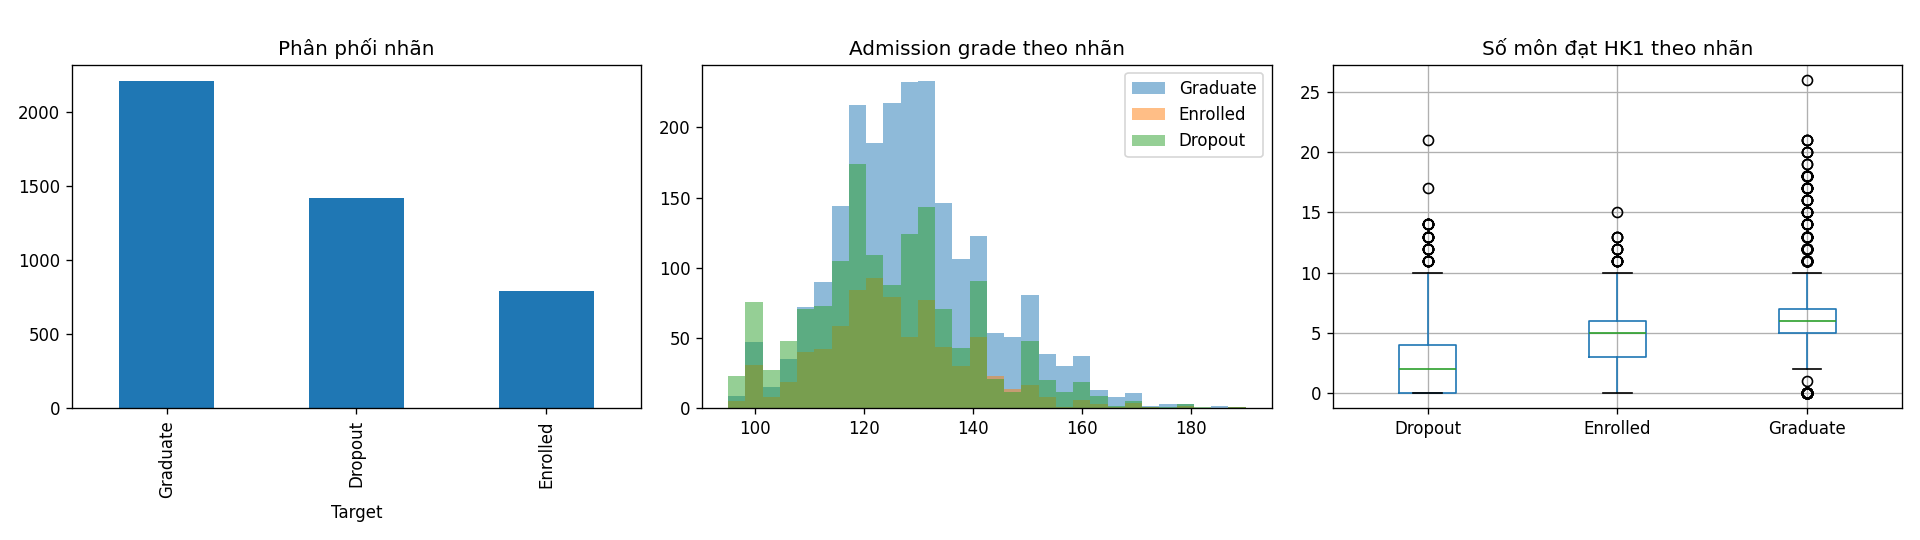
\includegraphics[width=\textwidth]{eda_overview.png}
\caption{Tổng quan EDA: phân phối nhãn, điểm trúng tuyển và số môn đạt học kỳ 1}
\label{fig:eda}
\end{figure}

\paragraph{Thống kê mô tả các biến số.} Bảng \ref{tab:desc} tóm tắt các biến số chính. Chỉ số ``Ngoại lệ (\%)'' là tỷ lệ giá trị nằm ngoài khoảng $[Q_1 - 1{,}5\,\text{IQR};\ Q_3 + 1{,}5\,\text{IQR}]$.

\begin{table}[H]
\centering
\caption{Thống kê mô tả một số biến số}
\label{tab:desc}
\small
\begin{tabular}{>{\raggedright\arraybackslash}p{4.6cm}*{5}{>{\raggedleft\arraybackslash}p{2.0cm}}}
\toprule
Biến & Trung bình & Độ lệch chuẩn & Trung vị & Độ lệch (skew) & Ngoại lệ (\%) \\
\midrule
\texttt{Age at enrollment} & 23.27 & 7.59 & 20 & 2.05 & 9.97 \\
\texttt{Admission grade} & 126.98 & 14.48 & 126.1 & 0.53 & 1.94 \\
\texttt{Previous qualification (grade)} & 132.61 & 13.19 & 133.1 & 0.31 & 4.05 \\
\texttt{1st sem (approved)} & 4.71 & 3.09 & 5 & 0.77 & 4.07 \\
\texttt{1st sem (grade)} & 10.64 & 4.84 & 12.29 & $-1.57$ & 16.41 \\
\texttt{2nd sem (approved)} & 4.44 & 3.01 & 5 & 0.31 & 0.99 \\
\texttt{2nd sem (grade)} & 10.23 & 5.21 & 12.20 & $-1.31$ & 19.82 \\
\bottomrule
\end{tabular}
\end{table}

Nhìn vào Bảng \ref{tab:desc} có ba nhận xét. Thứ nhất, tuổi khi nhập học lệch phải mạnh (skew 2.05, tối đa 70 tuổi) với gần 10\% là ngoại lệ theo quy tắc IQR. Các giá trị này nằm trong miền hợp lệ của từ điển dữ liệu nên nhóm giữ lại; dữ liệu không cho biết chắc chắn đây có phải sinh viên đi học lại hay không. Thứ hai, các biến điểm trung bình và số môn đạt có phân phối lệch trái, tức phần lớn sinh viên đạt điểm khá cao và chỉ một nhóm nhỏ có điểm thấp. Thứ ba, các biến này có thang đo khác nhau (điểm từ 0--20, số môn đếm được, điểm trúng tuyển từ 95 đến 190), nên cần chuẩn hóa cho K-NN và Naive Bayes. Đây là lý do Luồng A và Luồng B đều có bước chuẩn hóa.

\paragraph{Biến phân loại và biến gần như hằng số.} Trong mã nguồn có 9 cột phân loại đa giá trị (\texttt{CAT\_COLS}) được mã hóa one-hot và 8 cột nhị phân 0/1 (\texttt{BIN\_COLS}). Hai nhóm vấn đề cần lưu ý:
\begin{itemize}[leftmargin=2em]
\item \textbf{Biến gần như hằng số.} \texttt{Nationality} có 97.5\% sinh viên mang quốc tịch Bồ Đào Nha (mã 1); \texttt{International} có 97.5\% giá trị 0; \texttt{Educational special needs} có 98.8\% giá trị 0. Các biến này chứa rất ít thông tin phân biệt, nên nhóm giữ lại trong pipeline nhưng kỳ vọng đóng góp nhỏ vào dự đoán.
\item \textbf{Mã hiếm.} \texttt{Nationality} có 16 giá trị xuất hiện dưới 10 lần. Các giá trị này được gom vào một nhóm chung bằng tham số \texttt{min\_frequency=10} của one-hot encoder. Biến \texttt{Course} có 17 khóa học và không có khóa nào dưới 10 mẫu, nên không cần gom.
\end{itemize}
Ngoài ra, ba biến vĩ mô (thất nghiệp, lạm phát, GDP) chỉ có khoảng 9--10 giá trị khác nhau trên toàn bộ dữ liệu, vì mỗi năm nhập học có một giá trị chung cho mọi sinh viên. Điều này khớp với lập luận ở Bảng \ref{tab:flow} về việc loại các biến này khỏi Luồng B.

\paragraph{Mối liên hệ với nhãn bỏ học.} Bảng \ref{tab:med} so sánh trung vị của một số biến theo nhãn. Khoảng cách giữa nhóm bỏ học và nhóm tốt nghiệp rất rõ, đặc biệt ở học kỳ 2.

\begin{table}[H]
\centering
\caption{Trung vị của một số biến theo nhãn \texttt{Target}}
\label{tab:med}
\begin{tabular}{lrrr}
\toprule
Biến & Bỏ học & Đang học & Tốt nghiệp \\
\midrule
Số môn đạt học kỳ 1 & 2 & 5 & 6 \\
Số môn đạt học kỳ 2 & 0 & 4 & 6 \\
Điểm trung bình học kỳ 1 & 10.93 & 12.00 & 13.00 \\
Điểm trung bình học kỳ 2 & 0.00 & 12.00 & 13.00 \\
Điểm trúng tuyển & 123.6 & 124.1 & 127.4 \\
Tuổi khi nhập học & 23 & 20 & 19 \\
\bottomrule
\end{tabular}
\end{table}

Hình \ref{fig:hist} cho thấy phân phối của các biến theo từng nhóm. Nhóm bỏ học tập trung ở số môn đạt thấp và tuổi cao hơn, nhưng vùng chồng lấp giữa hai nhóm vẫn lớn, nên không có ngưỡng nào tách hoàn toàn hai nhóm. Hình \ref{fig:box} thể hiện rõ hơn qua box plot.

\begin{figure}[H]
\centering
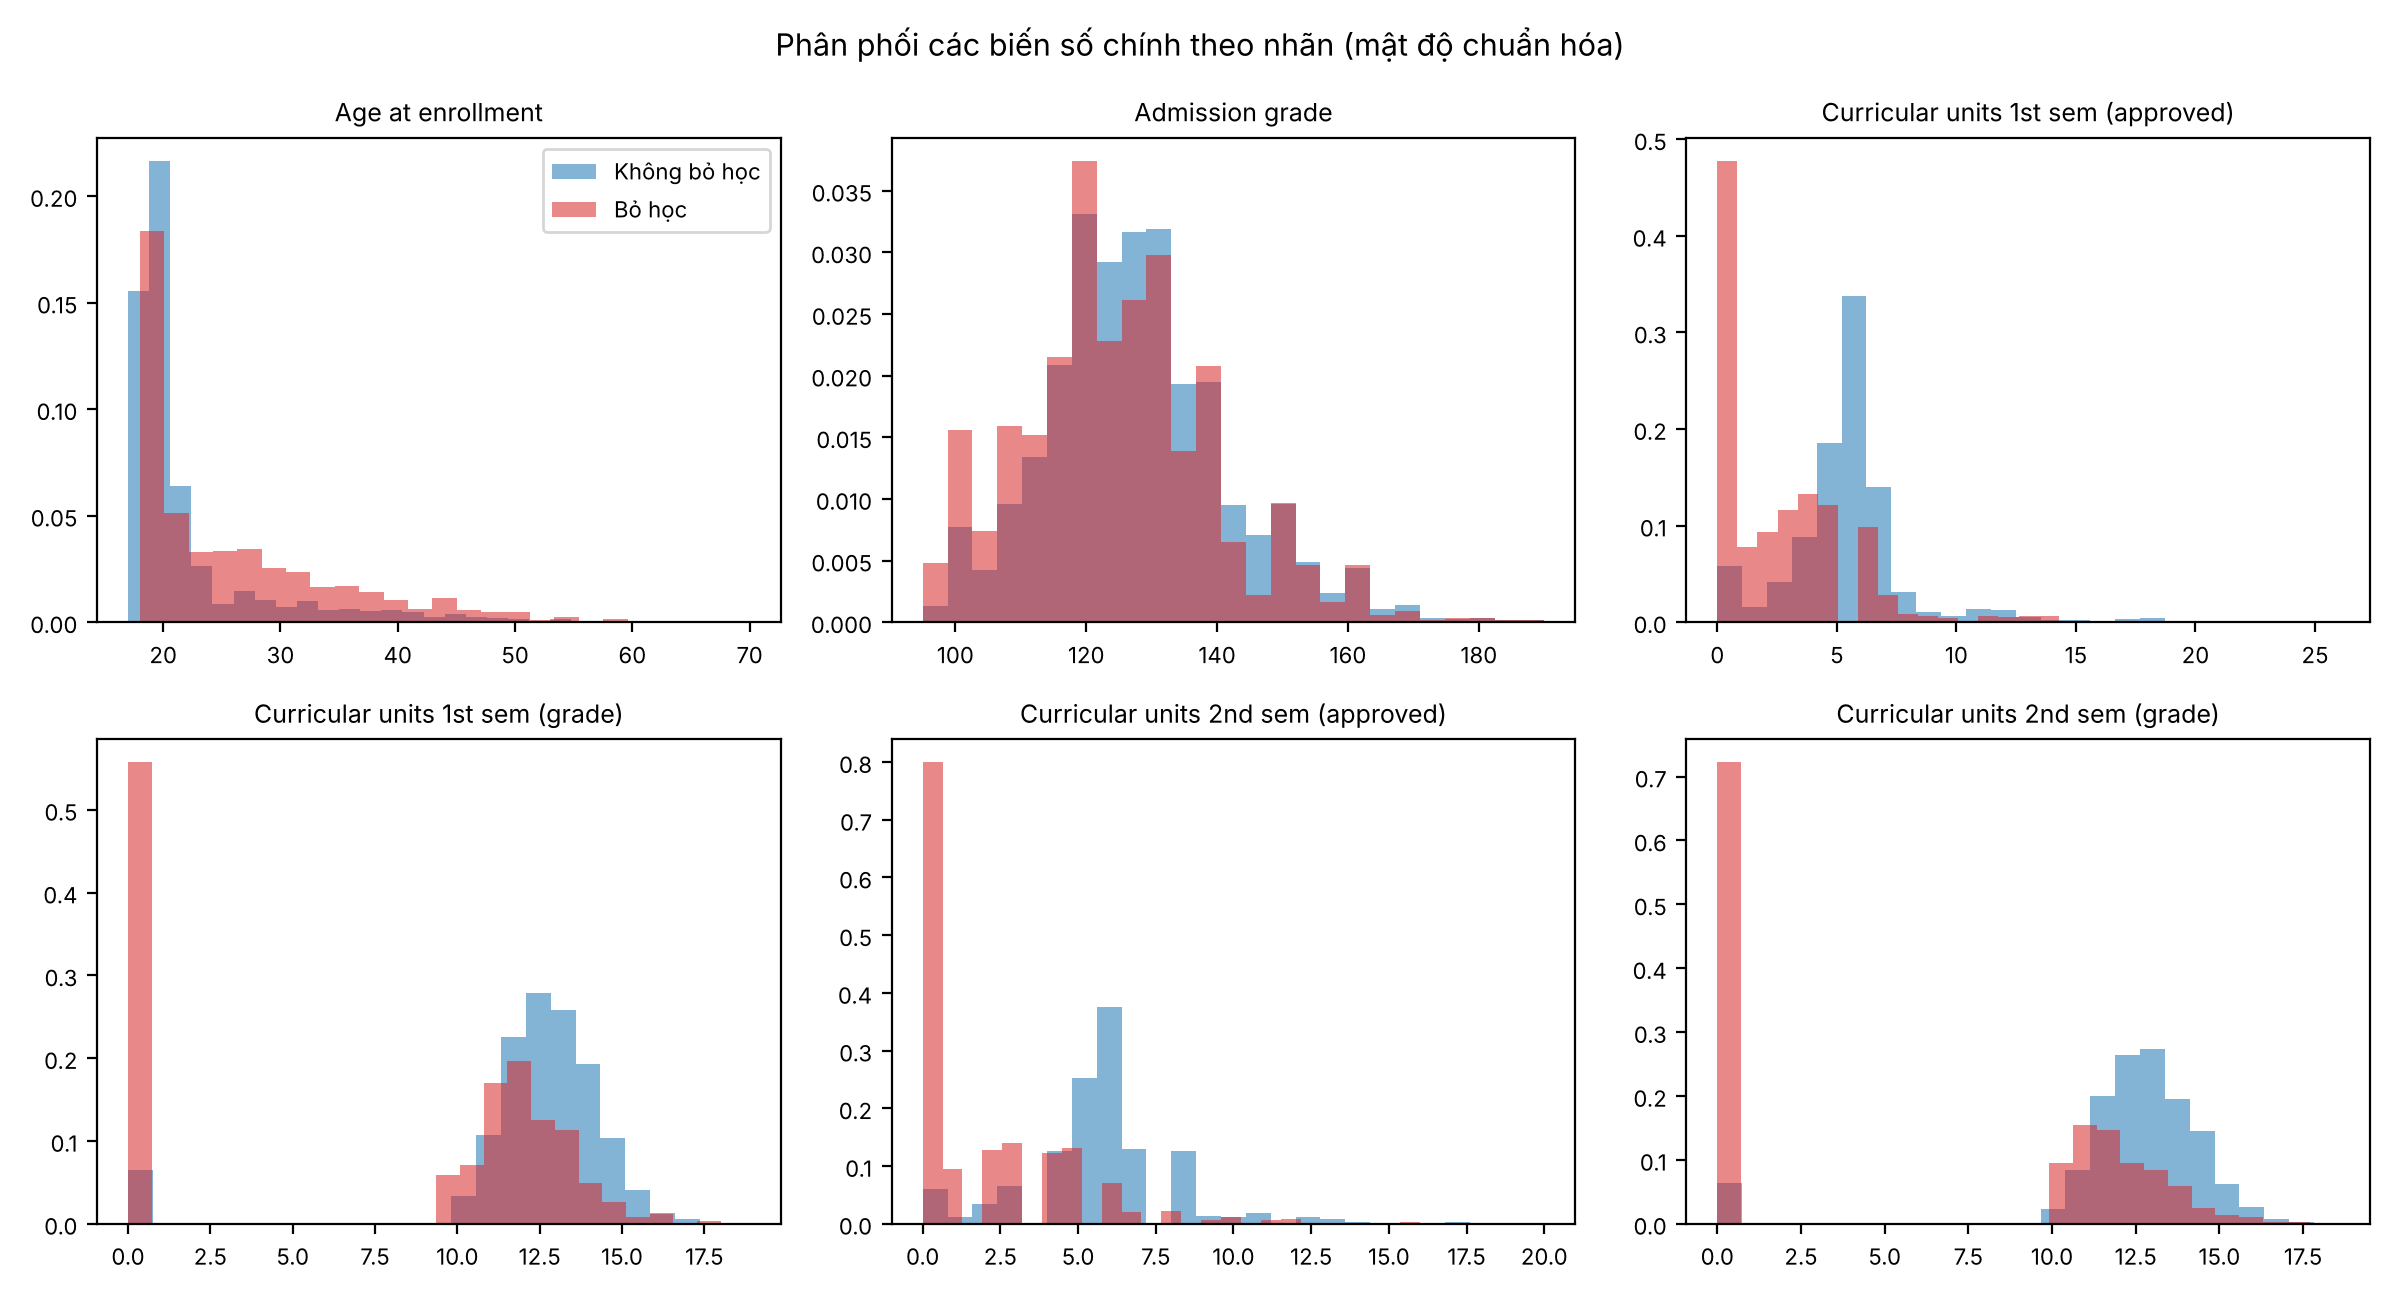
\includegraphics[width=\textwidth]{eda_hist_numeric.png}
\caption{Phân phối các biến số chính theo nhãn bỏ học (mật độ chuẩn hóa)}
\label{fig:hist}
\end{figure}

\begin{figure}[H]
\centering
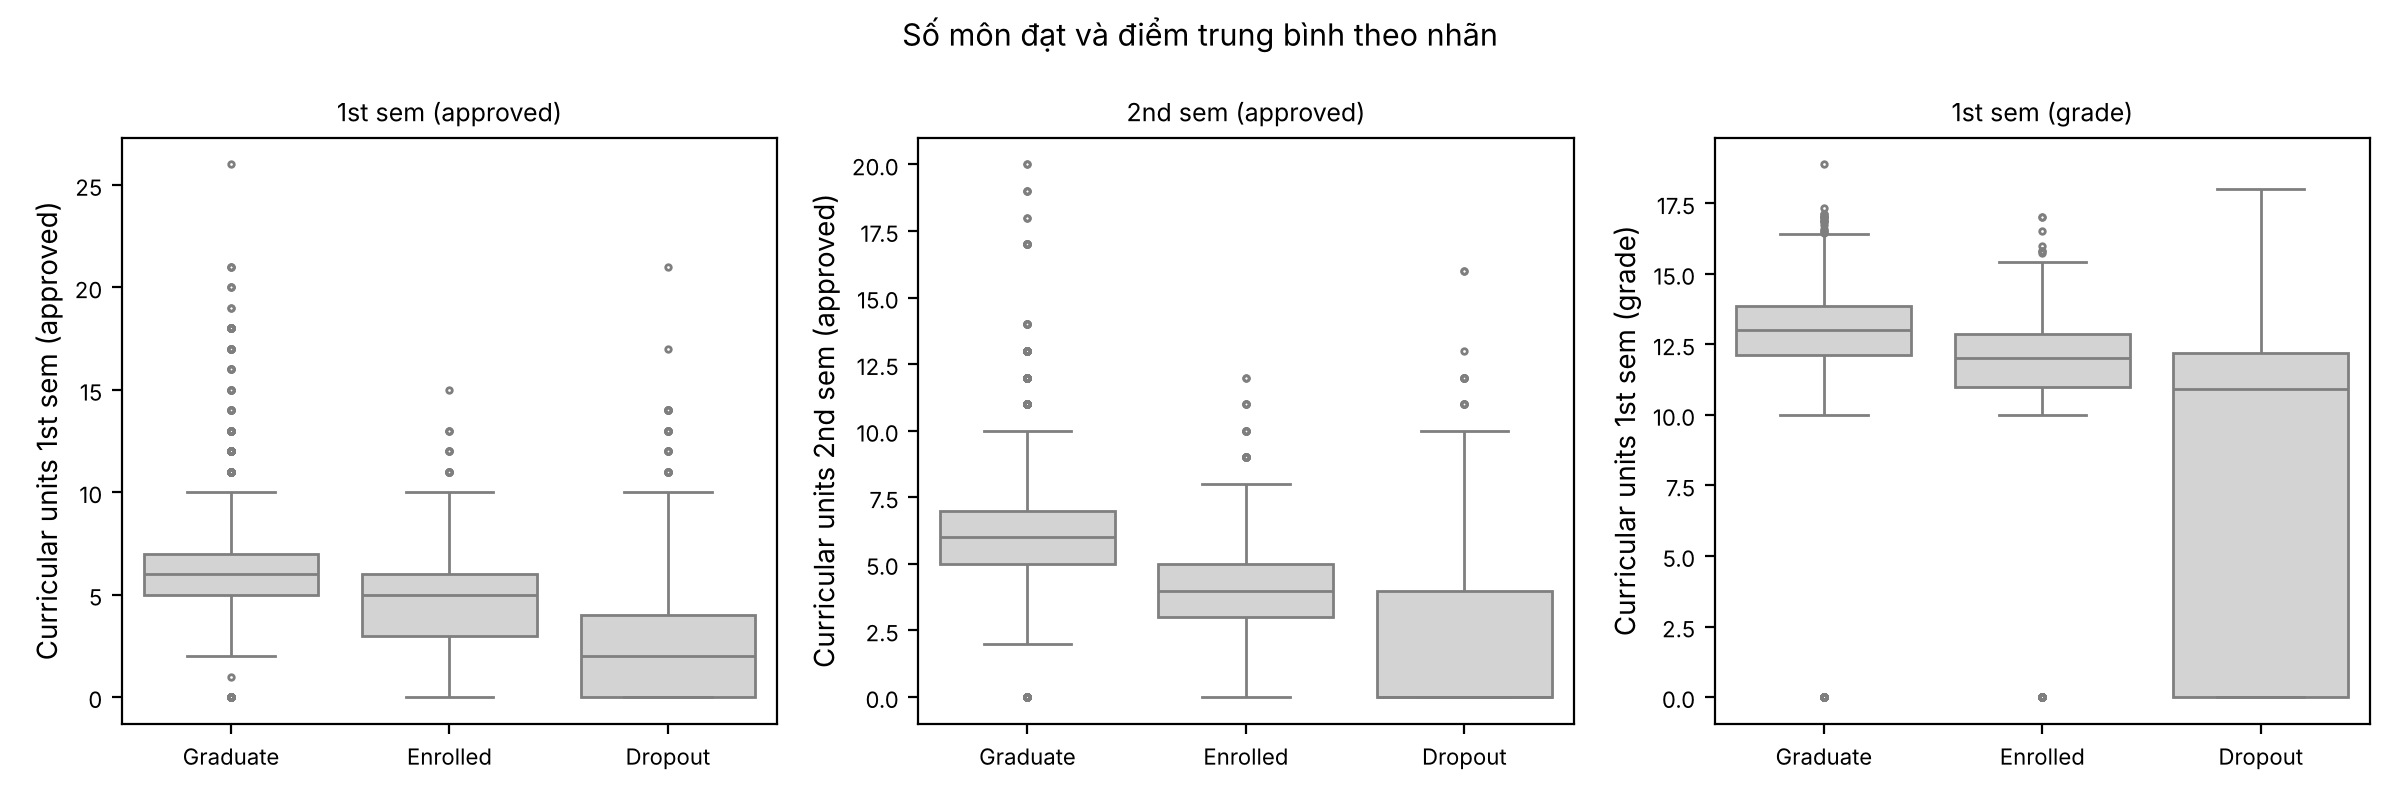
\includegraphics[width=\textwidth]{eda_box_by_target.png}
\caption{Số môn đạt và điểm trung bình theo nhãn \texttt{Target}}
\label{fig:box}
\end{figure}

Hình \ref{fig:rate} cho thấy tỷ lệ bỏ học theo các biến nhị phân về tài chính và giới tính. Sinh viên có nợ học phí có tỷ lệ bỏ học 62.0\%, so với 28.3\% ở nhóm không nợ. Nhóm chưa đóng học phí đúng hạn có tỷ lệ 86.6\%, trong khi nhóm đóng đúng hạn chỉ 24.7\%. Sinh viên có học bổng có tỷ lệ 12.2\%, thấp hơn đáng kể so với 38.7\% ở nhóm không có. Tỷ lệ bỏ học của nam (45.1\%) cao hơn nữ (25.1\%). Các biến tài chính có liên hệ mạnh nhất với nhãn trong số các biến nhị phân.

\begin{figure}[H]
\centering
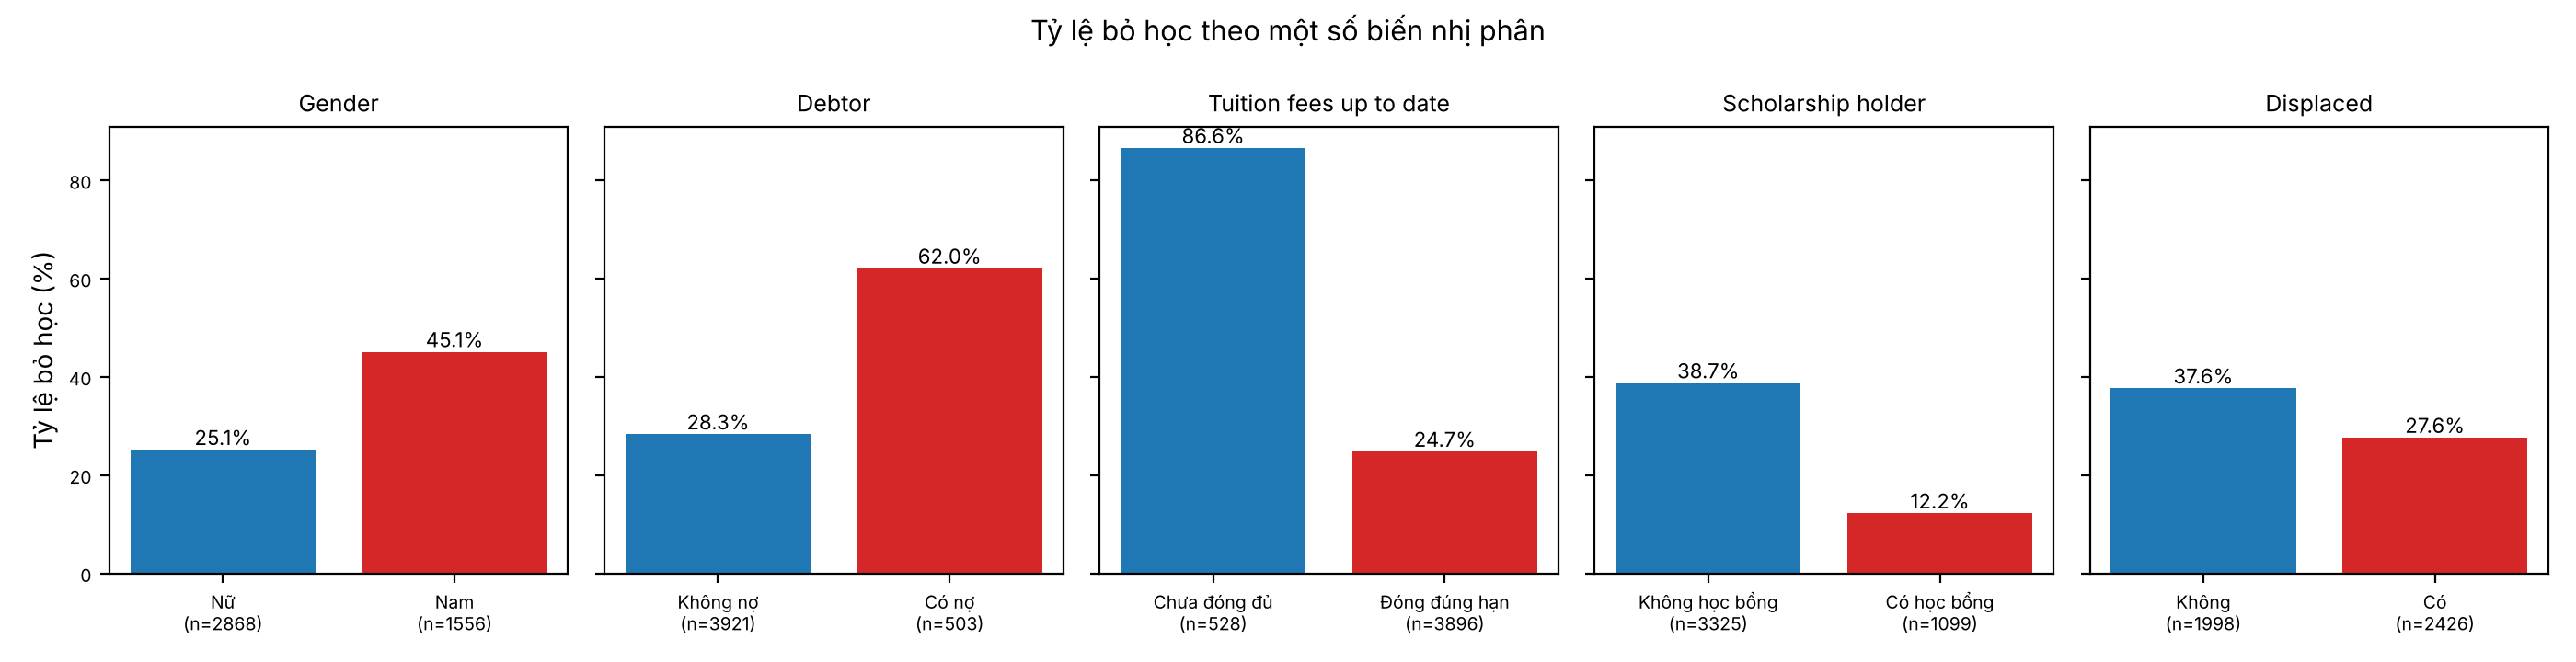
\includegraphics[width=\textwidth]{eda_rate_binary.png}
\caption{Tỷ lệ bỏ học theo một số biến nhị phân}
\label{fig:rate}
\end{figure}

\paragraph{Tương quan giữa các biến.} Hình \ref{fig:corr} thể hiện ma trận tương quan Spearman, phù hợp hơn Pearson vì nhiều biến lệch và có giá trị rời rạc. Ba nhận xét chính:
\begin{itemize}[leftmargin=2em]
\item \textbf{Dư thừa giữa các học kỳ.} Các biến cùng loại ở học kỳ 1 và học kỳ 2 tương quan rất mạnh, ví dụ số môn tín chỉ được công nhận (0.95), số môn đăng ký (0.94) và số môn đạt (0.90). Các đặc trưng này mang gần như cùng thông tin. Luồng B bổ sung thêm các tỷ lệ theo từng dòng nhưng vẫn giữ các biến thô, nên dư thừa vẫn còn trong Luồng B.
\item \textbf{Dư thừa giữa nghề nghiệp cha và mẹ.} Hai biến \texttt{Mother's occupation} và \texttt{Father's occupation} có tương quan 0.91, nên một trong hai có thể bỏ đi mà không làm mất nhiều thông tin. Nhóm giữ cả hai vì chưa kiểm tra riêng ảnh hưởng của từng biến.
\item \textbf{Tương quan với nhãn.} Các biến có tương quan âm mạnh nhất với \texttt{y} là số môn đạt học kỳ 2 ($-0.57$), số môn đạt học kỳ 1 ($-0.48$) và điểm trung bình học kỳ 1 ($-0.48$). Tuổi khi nhập học ($+0.25$) và hình thức đăng ký ($+0.20$) có tương quan dương yếu hơn. Các biến vĩ mô và nhân khẩu học khác gần như không tương quan với nhãn ($|\rho| < 0.1$).
\end{itemize}

\begin{figure}[H]
\centering
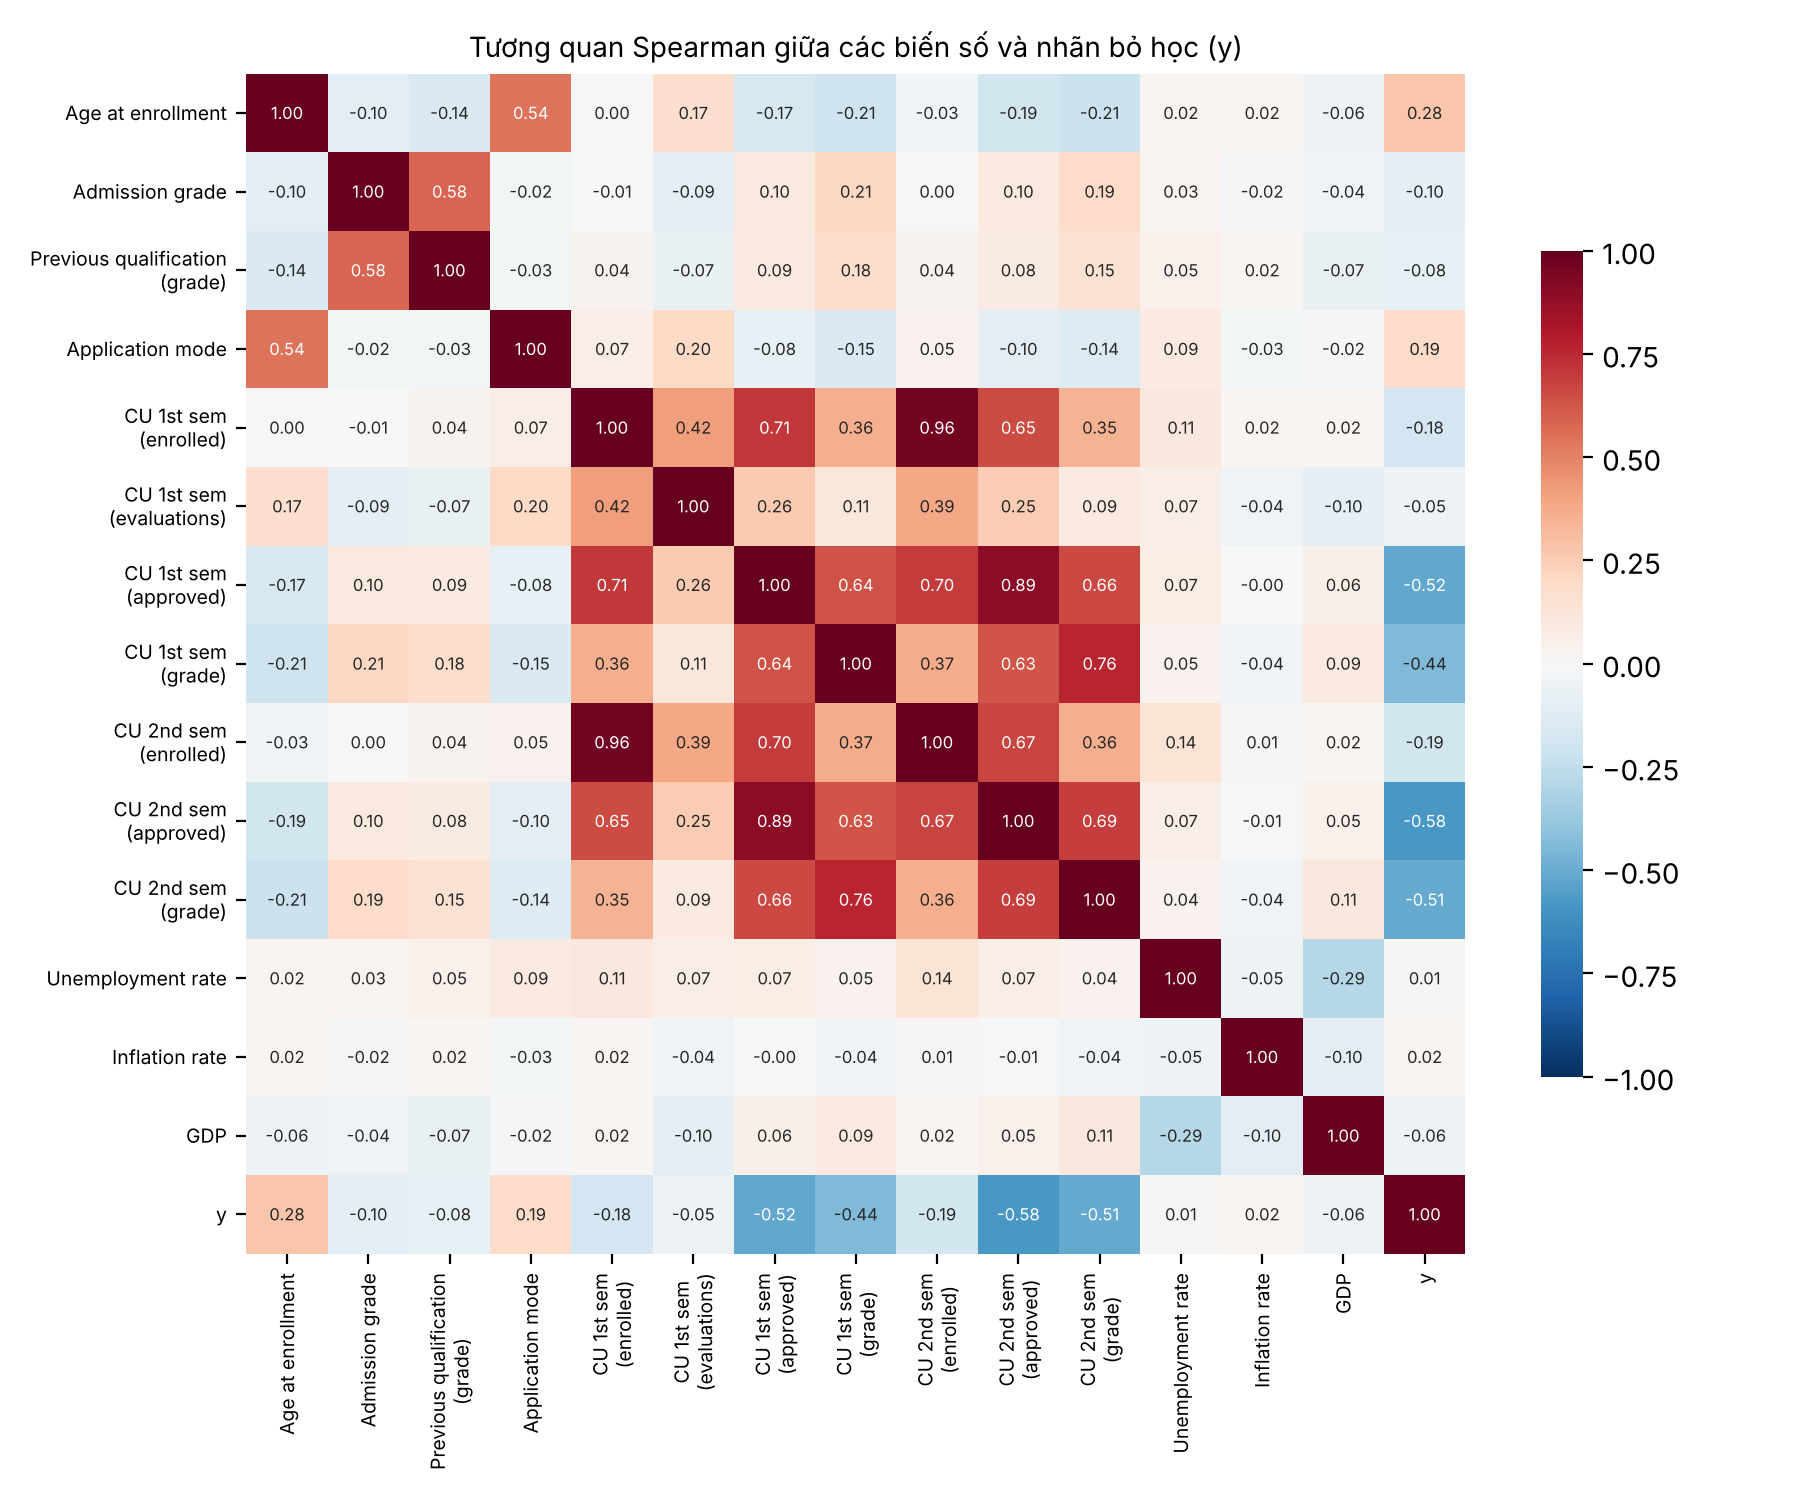
\includegraphics[width=0.85\textwidth]{eda_corr.png}
\caption{Ma trận tương quan Spearman giữa các biến số và nhãn bỏ học \texttt{y}}
\label{fig:corr}
\end{figure}

\paragraph{Phân tích rò rỉ dữ liệu.} Nhóm rà soát từng nhóm biến để xác định khả năng rò rỉ thông tin từ nhãn vào đặc trưng:
\begin{itemize}[leftmargin=2em]
\item \textbf{Biến nhân khẩu học, học vấn đầu vào, tài chính và vĩ mô}: được ghi nhận trước hoặc tại thời điểm nhập học, không phụ thuộc vào kết quả cuối cùng. Các biến này được giữ lại.
\item \textbf{Học kỳ 1}: được ghi nhận khi kết thúc học kỳ 1, trước thời điểm cảnh báo. Các biến này được giữ lại trong phạm vi \texttt{early}.
\item \textbf{Học kỳ 2}: dữ liệu có sau khi học kỳ 2 kết thúc. Trung vị số môn đạt học kỳ 2 của nhóm bỏ học bằng 0, so với 6 ở nhóm tốt nghiệp. Tuy nhiên đây không phải rò rỉ nhãn theo nghĩa kỹ thuật, vì dữ liệu được ghi trước khi nhãn cuối cùng được xác định. Vấn đề ở đây là dữ liệu đến quá muộn để can thiệp. Vì vậy học kỳ 2 chỉ được đưa vào phạm vi \texttt{full} để so sánh.
\end{itemize}
Trong 1421 sinh viên bỏ học, có 77 em không có đăng ký môn nào ở học kỳ 1; trong 3003 sinh viên không bỏ học, có 103 em không có đăng ký môn nào ở học kỳ 2. Các con số này cho thấy việc không đăng ký môn chưa phải là dấu hiệu đủ để xác định sinh viên đã bỏ học, nên nhóm không dùng riêng điều kiện này làm quy tắc.

\paragraph{Kết luận từ EDA.} Từ các phân tích trên, nhóm rút ra ba giả thuyết dùng cho giai đoạn mô hình:
\begin{enumerate}[leftmargin=2em]
\item Kết quả học tập học kỳ 1 và các biến tài chính (nợ học phí, học phí đúng hạn, học bổng) là những tín hiệu mạnh nhất cho nguy cơ bỏ học.
\item Các đặc trưng dạng tỷ lệ theo số môn đăng ký có thể cải thiện so với số đếm thô, vì giảm ảnh hưởng của việc sinh viên đăng ký số môn khác nhau.
\item Các biến vĩ mô và các biến gần như hằng số có đóng góp nhỏ, nên việc bỏ chúng có thể giúp giảm nhiễu cho K-NN.
\end{enumerate}
Các giả thuyết này được kiểm chứng ở Bảng \ref{tab:results} và Bảng \ref{tab:full}.

% ------------------------------------------------------------------
% 2. THIẾT KẾ GIẢI PHÁP VÀ QUY TRÌNH HỌC MÁY
% ------------------------------------------------------------------
\section{Thiết kế giải pháp và quy trình học máy}

\subsection{Sơ đồ pipeline tổng quát}
Quy trình của nhóm gồm các bước sau, từ dữ liệu thô đến kết quả:
\begin{enumerate}
  \item \textbf{Nạp và làm sạch:} đọc file, chuẩn hóa tên cột, loại dòng trùng, chuyển điểm 0 của môn không có đánh giá thành thiếu, tạo nhãn nhị phân $y$.
  \item \textbf{Kỹ thuật đặc trưng:} tạo đặc trưng tỷ lệ theo từng dòng (không học tham số nên không gây rò rỉ).
  \item \textbf{Chia dữ liệu:} tách tập huấn luyện và tập kiểm thử theo tỷ lệ 80:20, phân tầng theo nhãn.
  \item \textbf{Tiền xử lý trong pipeline:} điền thiếu, chuẩn hóa (nếu cần), mã hóa one-hot. Các bước này chỉ học trên tập huấn luyện.
  \item \textbf{Huấn luyện và chọn siêu tham số:} kiểm định chéo 5 lớp trên tập huấn luyện.
  \item \textbf{Đánh giá:} tính các độ đo trên tập kiểm thử, phân tích ma trận nhầm lẫn và lỗi.
\end{enumerate}

\subsection{Chia dữ liệu và hạn chế rò rỉ dữ liệu}
\begin{itemize}
  \item Tỷ lệ chia: 80\% huấn luyện (3539 mẫu), 20\% kiểm thử (885 mẫu), \texttt{stratify=y}, \texttt{random\_state=42}.
  \item Lựa chọn siêu tham số dùng \texttt{StratifiedKFold} với 5 lớp, \texttt{shuffle=True} và \texttt{random\_state=42} trên tập huấn luyện, với độ đo F1 của lớp bỏ học.
  \item Tập kiểm thử chỉ được dùng một lần để báo cáo kết quả cuối. Mô hình tốt nhất được chọn theo điểm CV, không chọn theo điểm kiểm thử.
  \item Các bước học tham số (điền giá trị thiếu bằng trung vị, chuẩn hóa, mã hóa) được đặt trong \texttt{Pipeline}, nên khi kiểm định chéo, mỗi fold chỉ học trên phần huấn luyện của fold đó.
  \item Các đặc trưng tỷ lệ chỉ là phép tính trên từng dòng, không phụ thuộc vào thống kê của toàn bộ dữ liệu, nên không gây rò rỉ.
\end{itemize}

\subsection{Hai phạm vi đặc trưng}
Nhóm thử nghiệm hai phạm vi đặc trưng để trả lời câu hỏi: \emph{có nên đợi đến hết học kỳ 2 mới cảnh báo hay không?}
\begin{itemize}
  \item \textbf{Phạm vi \texttt{early} (phiên bản chính):} thông tin lúc nhập học và kết thúc học kỳ 1.
  \item \textbf{Phạm vi \texttt{full} (so sánh):} thêm thông tin học kỳ 2. Đây là phương án có thể đạt kết quả cao hơn nhưng không kịp để can thiệp.
\end{itemize}

\subsection{Hai luồng tiền xử lý}
Theo yêu cầu đề bài, nhóm xây dựng hai luồng từ cùng một dữ liệu thô (Bảng \ref{tab:flow}).

\begin{table}[H]
\centering
\caption{So sánh Luồng A và Luồng B}
\label{tab:flow}
\begin{tabular}{p{2.6cm}p{5.4cm}p{5.4cm}}
\toprule
Tiêu chí & Luồng A: cơ bản & Luồng B: cải tiến \\
\midrule
Đặc trưng số & Toàn bộ biến số thô, kể cả 3 biến vĩ mô & Biến số thô, \textbf{bỏ 3 biến vĩ mô}, thêm đặc trưng tỷ lệ \\
Đặc trưng tỷ lệ & Không & Tỷ lệ môn đạt/đăng ký; tỷ lệ môn không có đánh giá/đăng ký; (phạm vi \texttt{full}) chênh lệch điểm hai học kỳ \\
Điền thiếu & Trung vị (số), mode (phân loại) & Giống Luồng A \\
Mã hóa phân loại & One-hot, gom nhóm hiếm ($<10$ mẫu) & Giống Luồng A \\
Chuẩn hóa & Có (cho K-NN và Naive Bayes) & Có (cho K-NN và Naive Bayes) \\
\bottomrule
\end{tabular}
\end{table}

\paragraph{Lý do thiết kế Luồng B.} Ba biến vĩ mô (thất nghiệp, lạm phát, GDP) chỉ mô tả vùng tại thời điểm nhập học, nên mọi sinh viên cùng năm nhập học có giá trị gần giống nhau. Chúng dễ tạo ra tương quan giả và làm nhiễu K-NN. Đặc trưng tỷ lệ phản ánh trực tiếp mức độ tiến bộ học tập, tức là thứ gắn chặt hơn với nguy cơ bỏ học.

\subsection{Thuật toán và tham số}
\begin{table}[H]
\centering
\caption{Các mô hình và lưới siêu tham số}
\label{tab:models}
\begin{tabular}{p{2.8cm}p{4.2cm}p{6.2cm}}
\toprule
Mô hình & Vai trò & Siêu tham số tìm kiếm \\
\midrule
Majority & Baseline: luôn dự đoán lớp đa số & Không \\
DT mặc định & Baseline: cây quyết định với cấu hình mặc định & Không \\
K-NN & Thuật toán đã học & \texttt{n\_neighbors} $\in\{3,5,9,15,21\}$; \texttt{weights} $\in\{$uniform, distance$\}$ \\
Naive Bayes & Thuật toán đã học & \texttt{var\_smoothing} $\in\{10^{-9},10^{-7},10^{-5},10^{-3}\}$ \\
Decision Tree & Thuật toán đã học & \texttt{max\_depth} $\in\{3,5,7,10,\text{None}\}$; \texttt{min\_samples\_leaf} $\in\{5,10,20,50\}$; \texttt{criterion} $\in\{$gini, entropy$\}$; \texttt{class\_weight} $\in\{$None, balanced$\}$ \\
\bottomrule
\end{tabular}
\end{table}

\paragraph{Lý do lựa chọn.} Các mô hình được cài đặt bằng thư viện scikit-learn \cite{sklearn}; cơ sở lý thuyết tham khảo từ \cite{hastie}.
\begin{itemize}
  \item \textbf{K-NN} là mô hình dựa trên khoảng cách, đơn giản và dễ giải thích, nhưng nhạy cảm với thang đo và nhiều chiều, nên cần chuẩn hóa và so sánh hai luồng.
  \item \textbf{Naive Bayes} giả định các đặc trưng độc lập có điều kiện, nhanh và ổn định với dữ liệu nhỏ. Nhóm dùng GaussianNB trên các đặc trưng đã chuẩn hóa và one-hot. Đây là một phép xấp xỉ vì one-hot không tuân theo phân phối Gauss, nên nhóm xem kết quả của mô hình này như một tham chiếu.
  \item \textbf{Cây quyết định} xử lý tốt cả biến số và biến phân loại, không cần chuẩn hóa, và cho phép xem độ quan trọng của đặc trưng. Tham số \texttt{class\_weight=balanced} giúp mô hình chú ý hơn đến lớp bỏ học.
\end{itemize}

\subsection{Chỉ số đánh giá}
Vì dữ liệu mất cân bằng và mục tiêu là phát hiện sớm sinh viên có nguy cơ, nhóm dùng:
\begin{itemize}
  \item \textbf{Recall} của lớp bỏ học: tỷ lệ sinh viên bỏ học được phát hiện.
  \item \textbf{Precision}: tỷ lệ cảnh báo đúng trong các cảnh báo đã đưa ra.
  \item \textbf{F1-score}: trung bình điều hòa của Precision và Recall, dùng làm độ đo chính để chọn siêu tham số.
  \item \textbf{ROC-AUC}: khả năng xếp hạng nguy cơ, không phụ thuộc vào ngưỡng quyết định.
  \item \textbf{Accuracy} và \textbf{ma trận nhầm lẫn}: để tham khảo và phân tích lỗi.
\end{itemize}

% ------------------------------------------------------------------
% 3. PHÂN TÍCH MÃ NGUỒN VÀ CHỨC NĂNG
% ------------------------------------------------------------------
\section{Phân tích mã nguồn và chức năng}

\subsection{Cấu trúc thư mục}
\begin{verbatim}
de-tai-8/
|-- README.md             # hướng dẫn cài đặt và chạy
|-- requirements.txt      # thư viện và phiên bản
|-- data.csv              # dữ liệu (nguồn UCI 697, xem README)
|-- dropout_pipeline.py   # toàn bộ pipeline: EDA, huấn luyện, đánh giá
|-- results/              # hình ảnh, bảng kết quả, phân tích lỗi
`-- report/               # mã nguồn LaTeX của báo cáo
\end{verbatim}

\subsection{Chức năng của các hàm chính}
\begin{table}[H]
\centering
\caption{Mô tả các hàm trong \texttt{dropout\_pipeline.py}}
\label{tab:funcs}
\begin{tabular}{p{4.6cm}p{9.2cm}}
\toprule
Hàm & Chức năng \\
\midrule
\texttt{load\_data} & Đọc CSV, làm sạch tên cột, loại trùng, chuyển điểm 0 thành thiếu, tạo nhãn $y$ \\
\texttt{eda} & In thống kê và vẽ tổng quan phân phối \\
\texttt{engineer} & Tạo đặc trưng tỷ lệ theo từng dòng \\
\texttt{feature\_sets} & Trả về danh sách cột theo phạm vi \texttt{early}/\texttt{full} và luồng A/B \\
\texttt{make\_preprocessor} & Xây \texttt{ColumnTransformer}: điền thiếu, chuẩn hóa, one-hot \\
\texttt{model\_specs} & Định nghĩa các mô hình và lưới siêu tham số \\
\texttt{fit\_one} & Huấn luyện một mô hình, chọn siêu tham số bằng CV nếu có lưới \\
\texttt{test\_metrics} & Tính các độ đo trên tập kiểm thử \\
\texttt{run\_experiments} & Chạy toàn bộ thí nghiệm, lưu bảng và hình \\
\texttt{error\_analysis} & Phân tích đặc điểm nhóm TP/TN/FN/FP của mô hình tốt nhất \\
\texttt{save\_confusion} & Vẽ và lưu ma trận nhầm lẫn \\
\texttt{save\_tree\_importance} & Vẽ và lưu độ quan trọng đặc trưng của cây quyết định \\
\texttt{main} & Đọc tham số dòng lệnh \texttt{--data}, \texttt{--out} và chạy toàn bộ quy trình \\
\bottomrule
\end{tabular}
\end{table}

\subsection{Đoạn mã quan trọng}
Đoạn mã dưới đây thể hiện cách hai luồng và pipeline được xây dựng. Toàn bộ mã nằm trong file \texttt{dropout\_pipeline.py}.

\begin{lstlisting}[caption={Xây dựng pipeline tiền xử lý và chọn cột theo luồng}]
def make_preprocessor(num_cols, cat_cols, scale):
    num_steps = [("imputer", SimpleImputer(strategy="median"))]
    if scale:
        num_steps.append(("scaler", StandardScaler()))
    cat_pipe = Pipeline([
        ("imputer", SimpleImputer(strategy="most_frequent")),
        ("onehot", OneHotEncoder(handle_unknown="ignore",
                                 min_frequency=10, sparse_output=False)),
    ])
    return ColumnTransformer([
        ("num", Pipeline(num_steps), num_cols),
        ("cat", cat_pipe, cat_cols),
    ])

def feature_sets(setting, flow):
    sems = SEM1_COLS + (SEM2_COLS if setting == "full" else [])
    num = BASE_NUM + BIN_COLS + sems
    if flow == "A":
        num = num + MACRO_COLS
    else:
        eng = ["1st sem approval rate", "1st sem no-eval ratio"]
        if setting == "full":
            eng += ["2nd sem approval rate", "2nd sem no-eval ratio",
                    "grade change"]
        num = num + eng
    return num, CAT_COLS
\end{lstlisting}

% ------------------------------------------------------------------
% 4. THỬ NGHIỆM VÀ KẾT QUẢ
% ------------------------------------------------------------------
\section{Thử nghiệm và kết quả}

\subsection{Thiết lập thí nghiệm}
\begin{itemize}
  \item Môi trường: Python 3.12.3, scikit-learn 1.9.1, pandas 3.0.6, NumPy 2.5.4. Chạy trên Ubuntu 24.04.
  \item Hạt giống ngẫu nhiên: \texttt{random\_state=42} cho chia dữ liệu, kiểm định chéo và các mô hình có tính ngẫu nhiên.
  \item Tổng số cấu hình: 2 phạm vi $\times$ 2 luồng $\times$ 5 mô hình (gồm 2 baseline).
\end{itemize}

\subsection{Phương án baseline}
Baseline gồm hai phương án: \textbf{Majority} (luôn dự đoán ``không bỏ học'') làm mốc tối thiểu, và \textbf{cây quyết định mặc định} làm mốc cho việc tinh chỉnh. Mọi mô hình tinh chỉnh phải vượt được baseline này mới có ý nghĩa.

\subsection{Bảng kết quả}
Bảng \ref{tab:results} trình bày kết quả trên tập kiểm thử với phạm vi \texttt{early} và hai luồng. Điểm CV-F1 là điểm kiểm định chéo trên tập huấn luyện, dùng để chọn mô hình.

\begin{table}[H]
\centering
\caption{Kết quả trên tập kiểm thử, phạm vi \texttt{early}}
\label{tab:results}
\small
\begin{tabular}{llcccccc}
\toprule
Luồng & Mô hình & CV-F1 & Accuracy & Precision & Recall & F1 & ROC-AUC \\
\midrule
A & Majority & 0.000 & 0.679 & 0.000 & 0.000 & 0.000 & 0.500 \\
A & DT mặc định & 0.653 & 0.792 & 0.675 & 0.680 & 0.677 & 0.762 \\
A & K-NN & 0.662 & 0.825 & 0.838 & 0.563 & 0.674 & 0.835 \\
A & Naive Bayes & 0.639 & 0.686 & 0.506 & 0.856 & 0.636 & 0.810 \\
A & Decision Tree & 0.735 & 0.825 & 0.695 & 0.810 & 0.748 & 0.881 \\
\midrule
B & DT mặc định & 0.664 & 0.779 & 0.653 & 0.662 & 0.657 & 0.748 \\
B & K-NN & 0.701 & 0.832 & 0.869 & 0.560 & 0.681 & 0.859 \\
B & Naive Bayes & 0.650 & 0.710 & 0.529 & 0.866 & 0.657 & 0.823 \\
B & Decision Tree & 0.748 & 0.842 & 0.728 & 0.810 & 0.767 & 0.893 \\
\bottomrule
\end{tabular}
\end{table}

\noindent Bảng \ref{tab:full} so sánh với phạm vi \texttt{full}, dùng để đánh giá giá trị thêm của dữ liệu học kỳ 2.

\begin{table}[H]
\centering
\caption{So sánh phạm vi \texttt{early} và \texttt{full} (F1 và ROC-AUC trên tập kiểm thử)}
\label{tab:full}
\begin{tabular}{llcccc}
\toprule
Mô hình & Luồng & F1 (early) & AUC (early) & F1 (full) & AUC (full) \\
\midrule
K-NN & A & 0.674 & 0.835 & 0.696 & 0.856 \\
K-NN & B & 0.681 & 0.859 & 0.723 & 0.889 \\
Naive Bayes & A & 0.636 & 0.810 & 0.678 & 0.832 \\
Naive Bayes & B & 0.657 & 0.823 & 0.695 & 0.847 \\
Decision Tree & A & 0.748 & 0.881 & 0.763 & 0.899 \\
Decision Tree & B & 0.767 & 0.893 & 0.768 & 0.917 \\
\bottomrule
\end{tabular}
\end{table}

\subsection{Siêu tham số tốt nhất}
\begin{table}[H]
\centering
\caption{Siêu tham số được chọn bằng kiểm định chéo cho từng mô hình (phạm vi \texttt{early})}
\label{tab:best}
\begin{tabular}{llp{8cm}}
\toprule
Luồng & Mô hình & Tham số tốt nhất \\
\midrule
A & K-NN & \texttt{n\_neighbors=5}, \texttt{weights=distance} \\
A & Naive Bayes & \texttt{var\_smoothing=1e-9} \\
A & Decision Tree & \texttt{max\_depth=5}, \texttt{min\_samples\_leaf=50}, \texttt{criterion=entropy}, \texttt{class\_weight=balanced} \\
B & K-NN & \texttt{n\_neighbors=9}, \texttt{weights=distance} \\
B & Naive Bayes & \texttt{var\_smoothing=1e-9} \\
B & Decision Tree & \texttt{max\_depth=7}, \texttt{min\_samples\_leaf=50}, \texttt{criterion=entropy}, \texttt{class\_weight=balanced} \\
\bottomrule
\end{tabular}
\end{table}

\subsection{Biểu đồ}
\begin{figure}[H]
\centering
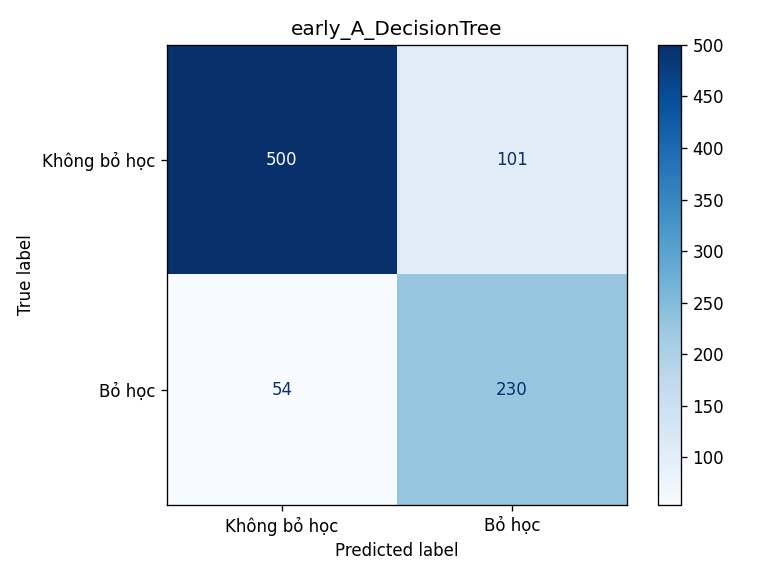
\includegraphics[width=0.48\textwidth]{cm_early_A_DecisionTree.png}
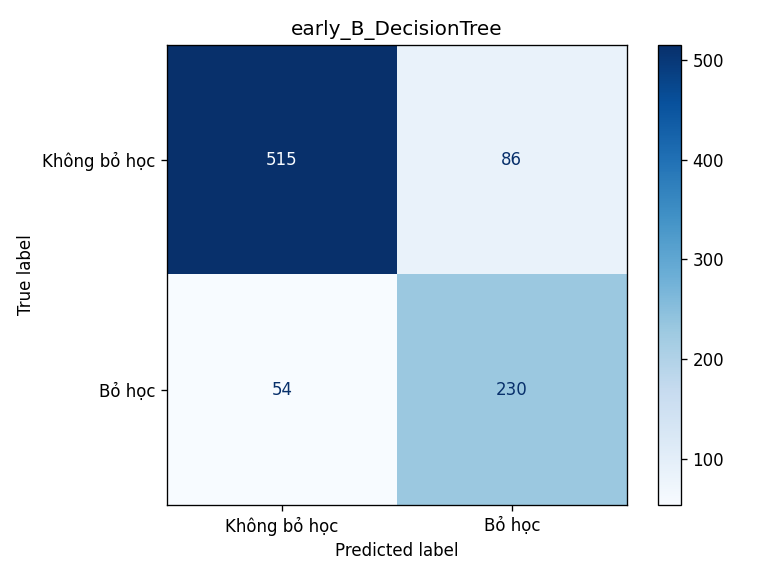
\includegraphics[width=0.48\textwidth]{cm_early_B_DecisionTree.png}
\caption{Ma trận nhầm lẫn của cây quyết định trên tập kiểm thử (trái: Luồng A; phải: Luồng B)}
\label{fig:cm}
\end{figure}

\begin{figure}[H]
\centering
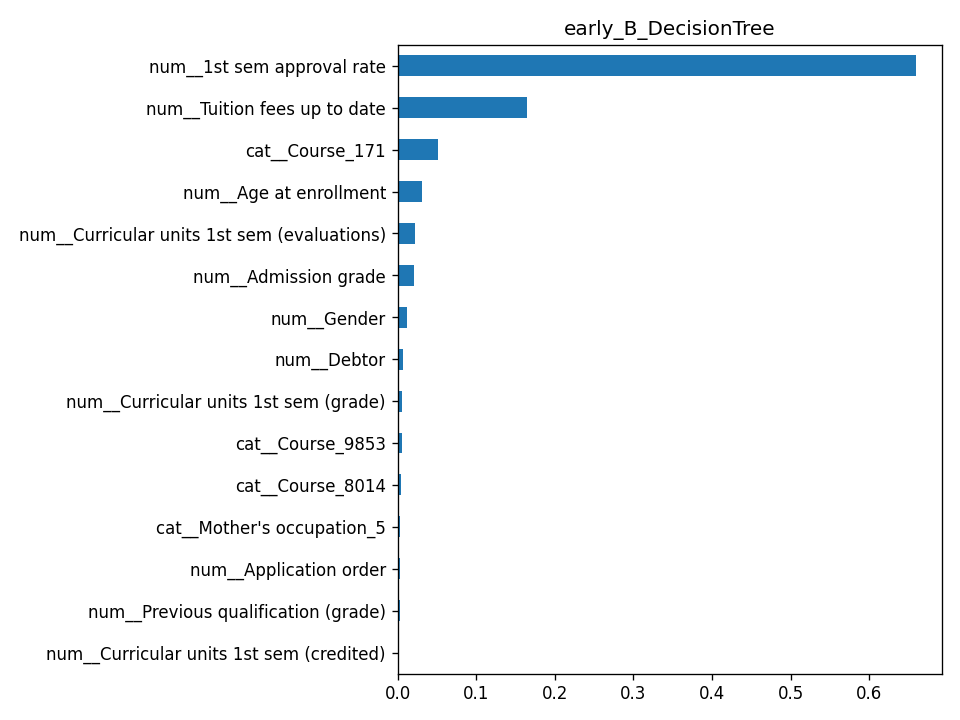
\includegraphics[width=0.7\textwidth]{importance_early_B_DecisionTree.png}
\caption{15 đặc trưng quan trọng nhất của cây quyết định tốt nhất (Luồng B)}
\label{fig:imp}
\end{figure}


% ------------------------------------------------------------------
% 5. THẢO LUẬN VÀ SO SÁNH
% ------------------------------------------------------------------
\section{Thảo luận và so sánh}

\subsection{So sánh ưu nhược điểm của các phương án}
\begin{itemize}
  \item \textbf{Majority:} Accuracy đạt 67.9\% nhưng Recall của lớp bỏ học bằng 0. Đây là ví dụ rõ nhất cho thấy Accuracy không đủ để đánh giá bài toán này.
  \item \textbf{K-NN:} F1 đạt 0.674 (Luồng A) và 0.681 (Luồng B), ROC-AUC 0.835 và 0.859. Mô hình có Precision cao nhất trong ba thuật toán (0.838–0.869) nhưng Recall thấp (khoảng 0.56), tức bỏ sót gần nửa số sinh viên bỏ học. Chuyển từ Luồng A sang B tăng CV-F1 từ 0.662 lên 0.701, phù hợp với giả thuyết rằng K-NN nhạy với các biến gần như hằng số. Hạn chế: phải lưu toàn bộ dữ liệu huấn luyện và chậm khi dự đoán với số lượng lớn.
  \item \textbf{Naive Bayes:} Mô hình có Recall cao nhất (0.856–0.866) nhưng Precision thấp nhất (0.506–0.529), nên Accuracy chỉ đạt 0.686–0.710, thấp hơn cả cây mặc định. F1 (0.636 và 0.657) thấp nhất trong ba thuật toán. Ưu điểm là nhanh và ổn định. Hạn chế là giả định độc lập có điều kiện thường không đúng với các đặc trưng học tập (ví dụ số môn đạt và điểm trung bình có tương quan mạnh).
  \item \textbf{Cây quyết định:} Đạt F1 cao nhất ở cả hai luồng: 0.748 (Luồng A) và 0.767 (Luồng B), ROC-AUC 0.881 và 0.893, Recall 0.810. Ưu điểm là dễ giải thích qua độ quan trọng đặc trưng. Hạn chế là dễ quá khớp nếu không giới hạn độ sâu.
\end{itemize}

\subsection{Vì sao một phương án hoạt động tốt hơn}
\paragraph{Luồng A so với Luồng B.} Ở phạm vi \texttt{early}, Luồng B cho F1 và ROC-AUC cao hơn Luồng A ở cả ba thuật toán (Bảng \ref{tab:results}): cây quyết định tăng F1 +0.019 và AUC +0.012, K-NN tăng +0.007 và +0.024, Naive Bayes tăng +0.021 và +0.013. Mức chênh lệch nhỏ và chỉ dựa trên một lần chia dữ liệu nên chưa thể khẳng định ý nghĩa thống kê. Hai thay đổi được áp dụng cùng lúc nên chưa tách riêng được đóng góp của từng thay đổi. Giải thích: các đặc trưng tỷ lệ giúp mô hình so sánh được sinh viên có số môn đăng ký khác nhau, điều mà số đếm thô không làm được. Việc bỏ biến vĩ mô giúp giảm nhiễu, đặc biệt có lợi cho K-NN vì khoảng cách không bị các biến gần như hằng số làm lệch.

\paragraph{Phạm vi \texttt{early} và \texttt{full}.} Thêm học kỳ 2 làm tăng ROC-AUC từ 0.018 đến 0.030 ở tất cả các mô hình và tăng F1 từ 0.001 (cây quyết định, Luồng B) đến 0.042 (K-NN Luồng B, Naive Bayes Luồng A) (Bảng \ref{tab:full}). Kết quả \texttt{full} thường cao hơn vì học kỳ 2 chứa rất nhiều thông tin về việc đã bỏ học hay chưa (ví dụ đăng ký ít môn hoặc không có đánh giá). Tuy nhiên, phiên bản này không còn hữu ích để cảnh báo sớm, nên nhóm chọn \texttt{early} làm kết quả chính.

\paragraph{Cây quyết định với \texttt{class\_weight}.} Ở phạm vi \texttt{early}, kiểm định chéo chọn \texttt{class\_weight=balanced} cho cả hai luồng, và Recall của lớp bỏ học đạt 0.810, cao hơn cây mặc định (0.680 và 0.662). Ở phạm vi \texttt{full}, cây chọn \texttt{class\_weight=None}, có Precision cao hơn (0.833 và 0.878) nhưng Recall thấp hơn (0.704 và 0.683). Đây là đánh đổi cần nêu rõ với nhà trường: bỏ sót sinh viên nguy cơ có chi phí cao hơn việc cảnh báo nhầm.

\subsection{Phân tích dự đoán sai}
Nhóm tách các mẫu theo bốn nhóm TP, TN, FN, FP và so sánh đặc điểm trung bình (file \texttt{error\_profile.csv}). Bảng \ref{tab:err} tổng hợp đặc điểm trung bình của bốn nhóm. Mô hình được phân tích là mô hình có CV-F1 cao nhất trên toàn bộ thí nghiệm: cây quyết định, Luồng B, phạm vi \texttt{full} (CV-F1 = 0.772, F1 = 0.768, ROC-AUC = 0.917).

\begin{table}[H]
\centering
\caption{Đặc điểm trung bình theo nhóm dự đoán (cây quyết định, Luồng B, phạm vi \texttt{full})}
\label{tab:err}
\begin{tabular}{lcccc}
\toprule
Đặc trưng & TP & TN & FN & FP \\
\midrule
Số môn đạt học kỳ 1 & 1.80 & 6.01 & 4.39 & 2.85 \\
Điểm TB học kỳ 1 & 7.01 & 12.83 & 12.27 & 10.25 \\
Điểm trúng tuyển & 123.18 & 128.39 & 126.79 & 123.87 \\
Tỷ lệ nợ học phí & 0.23 & 0.06 & 0.09 & 0.19 \\
Tỷ lệ đóng học phí đúng hạn & 0.53 & 0.98 & 0.93 & 0.78 \\
Tỷ lệ có học bổng & 0.08 & 0.34 & 0.16 & 0.15 \\
\bottomrule
\end{tabular}
\end{table}

\paragraph{Nhóm khó nhất: False Negative.} Sinh viên bỏ học nhưng bị dự đoán là không bỏ học có hồ sơ gần với nhóm TN hơn nhóm TP: số môn đạt học kỳ 1 là 4.39 (TN: 6.01; TP: 1.80), điểm trung bình học kỳ 1 là 12.27 (TN: 12.83; TP: 7.01), tỷ lệ đóng học phí đúng hạn 0.93 (TP: 0.53) và tỷ lệ nợ chỉ 0.09. Giả thuyết nguyên nhân: những sinh viên này có kết quả học kỳ 1 chưa đủ thấp để tách khỏi nhóm đang học, nên mô hình không phát hiện được. Các yếu tố như hoàn cảnh gia đình hoặc lý do cá nhân không có trong dữ liệu, đây là giới hạn của bài toán.

\paragraph{Nhóm False Positive.} Sinh viên bị cảnh báo nhầm có số môn đạt học kỳ 1 là 2.85, điểm trung bình 10.25, tỷ lệ nợ 0.19 và đóng học phí đúng hạn 0.78, gần với nhóm TP hơn, trong khi tỷ lệ có học bổng thấp (0.15). Trong thực tế, nhóm này vẫn có giá trị vì việc hỗ trợ thêm không gây hại lớn.

\paragraph{Khóa học dễ nhầm.} Ba khóa có nhiều False Negative nhất là mã 171 (18 trường hợp), 9853 (11) và 9500 (11); tiếp theo là mã 9670 (8). Điều này gợi ý tỷ lệ bỏ học khác nhau giữa các khóa, và mô hình chưa nắm bắt đầy đủ điều đó.

\subsection{Hạn chế}
\begin{itemize}
  \item \textbf{Dữ liệu:} chỉ thuộc một cơ sở đào tạo ở Bồ Đào Nha, giai đoạn cụ thể, nên khó tổng quát hóa cho môi trường khác, kể cả tại Việt Nam.
  \item \textbf{Thiếu biến quan trọng:} dữ liệu không có yếu tố tâm lý, thời gian đi làm thêm, khoảng cách từ nhà đến trường, hay sự hỗ trợ của gia đình.
  \item \textbf{Mất cân bằng lớp:} dù đã dùng F1, AUC và \texttt{class\_weight}, lớp bỏ học vẫn ít mẫu hơn, nên ước lượng Recall có độ không chắc chắn.
  \item \textbf{Ngưỡng quyết định:} nhóm dùng ngưỡng mặc định 0.5. Ngưỡng này nên được điều chỉnh theo chi phí thực tế của nhà trường.
  \item \textbf{Naive Bayes:} giả định chưa khớp với dữ liệu, nên kết quả chỉ mang tính tham khảo.
  \item \textbf{Đánh giá:} chỉ dùng một lần chia train/test. Kết quả có thể dao động khi đổi \texttt{random\_state}.
\end{itemize}

% ------------------------------------------------------------------
% 6. TỔNG KẾT VÀ HƯỚNG PHÁT TRIỂN
% ------------------------------------------------------------------
\section{Tổng kết và hướng phát triển}

\subsection{Tóm tắt kết quả chính}
\begin{enumerate}
  \item Dữ liệu gồm 4424 sinh viên, 32.1\% thuộc nhóm bỏ học. Dữ liệu sạch, nhưng điểm 0 của môn không có đánh giá cần được xử lý như giá trị thiếu.
  \item Với phạm vi cảnh báo sớm (\texttt{early}), mô hình tốt nhất là cây quyết định, Luồng B, đạt F1 0.767 và ROC-AUC 0.893 trên tập kiểm thử, vượt baseline Majority và cây mặc định.
  \item Luồng B tăng hiệu quả so với Luồng A ở mức +0.019 F1 và +0.012 ROC-AUC với cây quyết định, cho thấy đặc trưng tỷ lệ và việc bỏ biến vĩ mô có tác dụng nhẹ nhưng nhất quán ở cả ba thuật toán.
  \item Thêm dữ liệu học kỳ 2 giúp tăng ROC-AUC từ 0.018 đến 0.030 và F1 thêm từ 0.001 đến 0.042 tùy mô hình, nhưng không phù hợp để cảnh báo sớm.
\end{enumerate}

\subsection{Hướng cải tiến}
\begin{itemize}
  \item Điều chỉnh ngưỡng quyết định theo chi phí bỏ sót và chi phí cảnh báo nhầm, thay vì dùng 0.5.
  \item Thử các mô hình mạnh hơn như Random Forest hoặc gradient boosting, và so sánh với K-NN, Naive Bayes, Decision Tree đã học.
  \item Dùng CategoricalNB cho các biến phân loại thay vì GaussianNB trên one-hot.
  \item Thu thập thêm dữ liệu về yếu tố tâm lý, tài chính gia đình và thời gian làm thêm để cải thiện khả năng phát hiện các trường hợp FN.
  \item Đánh giá bằng nhiều lần chia (repeated stratified CV) để đo độ ổn định của kết quả.
\end{itemize}

% ------------------------------------------------------------------
% PHỤ LỤC
% ------------------------------------------------------------------
\appendix
\section{Khai báo sử dụng công cụ AI}
Nhóm có sử dụng công cụ AI (trợ lý lập trình và mô hình ngôn ngữ) để: (i) gợi ý cấu trúc mã nguồn và cách dùng \texttt{Pipeline} trong scikit-learn; (ii) kiểm tra lỗi cú pháp; (iii) hỗ trợ viết và chỉnh sửa văn bản báo cáo. Nhóm đã tự kiểm tra lại toàn bộ mã nguồn, chạy lại thí nghiệm và chịu trách nhiệm về nội dung, số liệu và các kết luận. Chi tiết được ghi trong file \texttt{AI\_USAGE.md} của repository.

\section{Hướng dẫn tái lập kết quả}
\begin{enumerate}
  \item Tải \texttt{data.csv} từ UCI 697 và đặt cùng thư mục với mã nguồn.
  \item Cài thư viện: \texttt{pip install -r requirements.txt}.
  \item Chạy: \texttt{python dropout\_pipeline.py --data data.csv --out results}.
  \item Kết quả nằm trong thư mục \texttt{results/}, khớp với các bảng và hình trong báo cáo.
\end{enumerate}

% ------------------------------------------------------------------
% TÀI LIỆU THAM KHẢO
% ------------------------------------------------------------------
\begin{thebibliography}{9}
\bibitem[Realinho et al.(2021)]{realinho2021}
Realinho, V., Machado, J., Baptista, L., \& Martins, M. V. (2021).
\textit{Predict Students' Dropout and Academic Success}. UCI Machine Learning Repository.
\url{https://archive.ics.uci.edu/dataset/697}

\bibitem{sklearn}
Pedregosa, F., et al. (2011). Scikit-learn: Machine Learning in Python. \textit{Journal of Machine Learning Research}, 12, 2825--2830.

\bibitem{hastie}
Hastie, T., Tibshirani, R., \& Friedman, J. (2009). \textit{The Elements of Statistical Learning}. Springer.
\end{thebibliography}

\end{document}
